\chapter{Conceptual Framework for GenAI-Driven Security Automation}

% TODO
% Sources of Security Data
% Quellen für alle Abschnitte hinzufügen
% TODO add references
% TOOD add diagramm

\section{Architectural Overview of the Proposed Framework}

This chapter introduces the conceptual framework designed to address the critical challenges of automated security analysis and policy generation for cloud infrastructure. The proposed architecture, illustrated in Figure~\ref{fig:prototype-architecture}, presents a comprehensive, multi-layered approach that systematically processes \gls{iac} artifacts and automatically generates corresponding security policies. At its core, the framework leverages the power of traditional static analysis tools and advanced \glspl{llm} to create a robust security automation pipeline.

\begin{figure}[htbp]
\centering
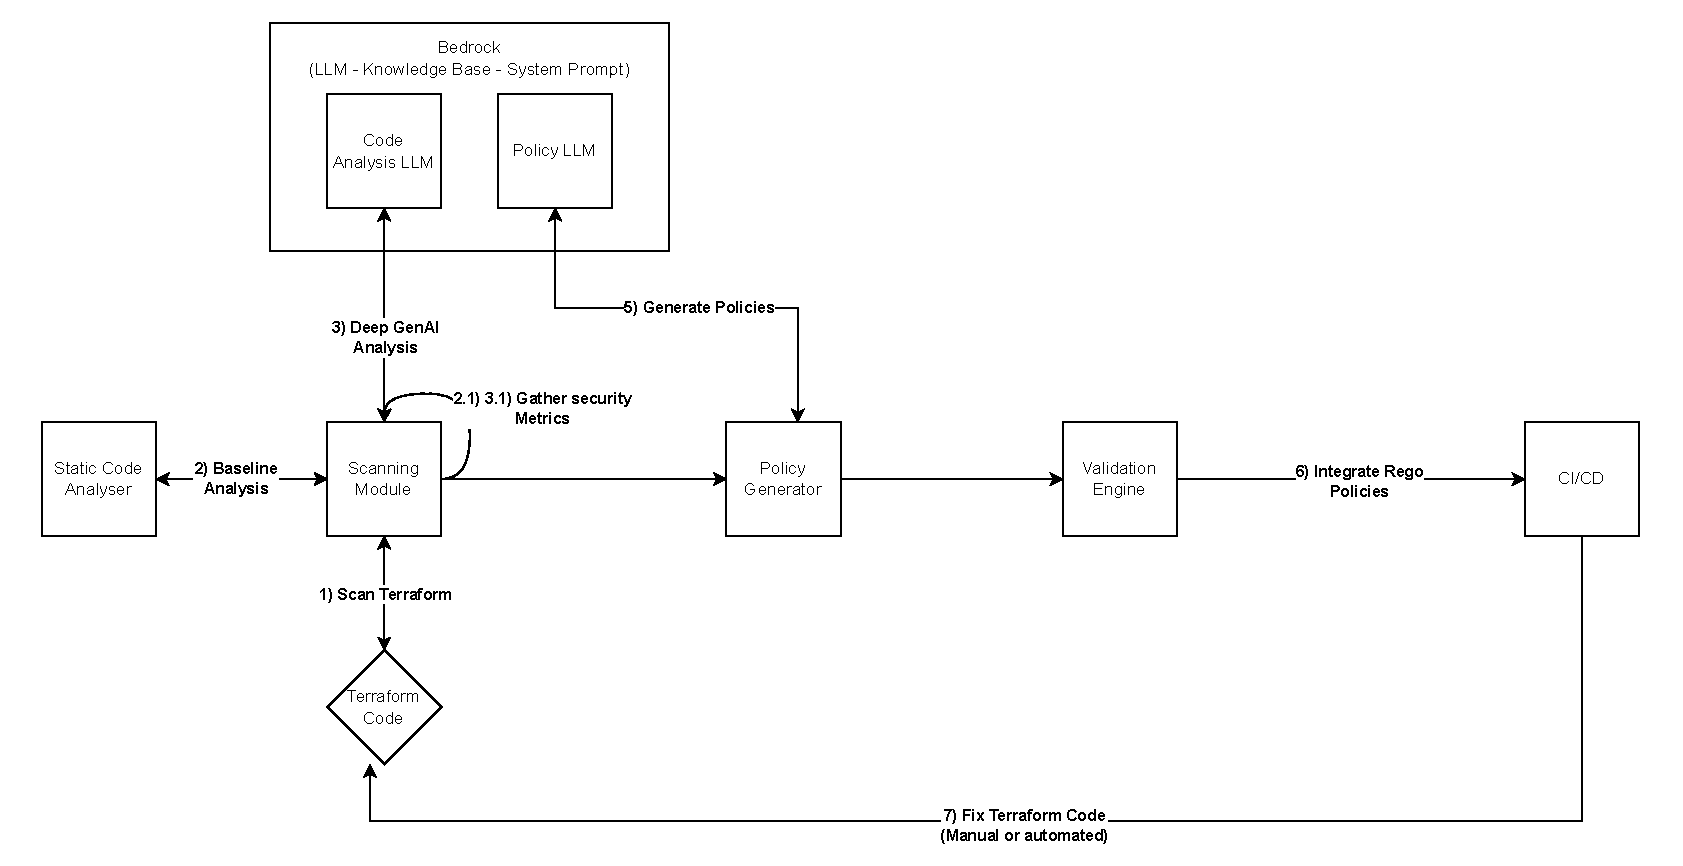
\includegraphics[width=\textwidth]{Figures/prototype.pdf}
\caption{Architectural Overview of the Proposed GenAI-Driven Security Automation Framework}
\label{fig:prototype-architecture}
\end{figure}

This hybrid model is intentionally designed for efficacy, combining the reliability of established security scanners for identifying known vulnerability patterns with the contextual intelligence of generative AI. This allows for deeper analytical capabilities, necessary for uncovering complex, context-dependent security issues that traditional tools often miss. Furthermore, the architecture is conceived for seamless integration into modern \gls{devops} workflows, particularly \gls{cicd} pipelines, to operationalize a Policy-as-Code model and enforce security throughout the development lifecycle.

The framework is organized into a logical pipeline comprising four distinct layers: the Data Ingestion Layer, the Data Processing Layer, the Code Generation Layer, and the Validation Layer. Each layer performs a specific function, building upon the output of the preceding one to create an end-to-end workflow. This process begins with the intake of infrastructure configuration definitions, proceeds through multi-stage static and AI-driven analysis, generates preventative security policies in a declarative, machine-readable format, and concludes with the rigorous validation of these AI-generated artifacts. This layered design aims to provide a comprehensive and efficient system for enhancing cloud security posture by translating identified vulnerabilities directly into enforceable controls. The following subsections will detail the specific roles and functions of each of these core layers.

\subsection{Data Ingestion Layer} % (fold)
\label{sec:data-ingestion-layer}

The Data Ingestion Layer serves as the foundational entry point for security artifacts into the automation framework. Its primary function is to ingest \gls{iac} configurations, a prevalent standard for provisioning and managing cloud infrastructure. The reliance on \gls{iac}, while enhancing automation and consistency, introduces significant risks such as misconfigurations, coding errors, and embedded secrets, making automated analysis a critical requirement for secure cloud operations \cite{hayagreevan_security_2024}.

This layer is designed to support both batch and real-time ingestion modes, a flexible approach that aligns with modern data pipeline architectures emphasizing scalability and performance \cite{ismail_big_2025}. Batch ingestion allows for comprehensive, scheduled scans of entire code repositories, while real-time ingestion facilitates immediate analysis within \gls{cicd} pipelines. The framework is designed to receive these \gls{iac} configurations via programmatic interfaces, ensuring seamless integration into existing developer workflows and automated systems.

Upon ingestion, the layer initiates a multi-stage preliminary analysis process. First, the raw \gls{iac} configuration is parsed for programmatic analysis. Following this step, a suite of established \gls{sast} tools is executed. This initial scan generates a baseline vulnerability report by checking the configurations against a comprehensive database of known misconfigurations, security vulnerabilities, and compliance violations. The structured output from this layer, comprising the original \gls{iac} configuration, its parsed representation, and the baseline vulnerability report, is then passed to the Data Processing Layer for the deeper, context-aware analysis powered by generative AI that is the focus of this research. In the following, the processes of the Data processing layer are explained more in Detail.

% subsubsection Data Ingestion Layer (end)

\section{Data Processing Layer}
\label{sec:data-processing-layer}

Following the Data Ingestion Layer, the Data Processing Layer is responsible for the core analysis of the ingested \gls{iac} artifacts. A central design principle of this framework is the segregation of processing activities into two distinct but complementary sub-layers: a traditional Static Analysis Engine and an advanced \gls{genai} Analysis Engine.

The rationale for this dual-layer architecture is to create a highly efficient and comprehensive security analysis pipeline. This approach leverages the respective strengths of each technology. Static analysis provides a rapid, reliable, and computationally inexpensive method for identifying a wide range of known, pattern-based vulnerabilities. By filtering out these common issues first, the framework can then employ the more resource-intensive \gls{genai} engine to focus on complex, context-dependent security flaws that traditional tools are ill-equipped to detect. This layered methodology optimizes analytical depth while maintaining operational efficiency, ensuring that both well-defined and nuanced vulnerabilities are addressed.

The first stage of this layer employs a suite of established \gls{sast} tools to conduct an initial scan of the \gls{iac} configuration. This engine examines the configuration for syntactic and structural flaws by referencing curated databases of known vulnerabilities, common misconfigurations, and code smells. It validates the configuration against established security benchmarks and standards. The primary output of this stage is a baseline vulnerability report, which provides a structured list of potential issues identified through deterministic, rule-based pattern matching. This report serves as a foundational input for the subsequent, more sophisticated analysis stage.

The second stage is the \gls{genai} Analysis Engine, which represents the core innovation of this framework and directly addresses the research interest in applying generative \gls{ai} to cloud security. This engine utilizes \glspl{llm} to perform a deeper, contextual analysis that transcends the limitations of traditional static scanners\cite{hayagreevan_security_2024, ling_enhancing_2024}. It takes as input both the original \gls{iac} configuration and the baseline vulnerability report from the previous stage, using the initial findings to enrich its analytical context.

This engine is designed to identify security weaknesses that require an understanding of developer intent, architectural relationships, and complex business logic\cite{noseevich_towards_2015}. Its capabilities include:

\begin{itemize}
\item \textbf{Identifying Context-Sensitive Flaws:} Detecting risks that emerge from the interaction of multiple configurations, such as overly permissive network rules that appear acceptable in isolation but create a vulnerability when combined with a specific resource's placement within the network architecture\cite{noseevich_towards_2015}.
\item \textbf{Uncovering Logical and Policy Violations:} Identifying logical flaws in resource deployments, such as potential circular dependencies, or violations of complex, unwritten organizational policies like nuanced tagging and naming conventions.
\item \textbf{Reducing False Positives:} Differentiating between genuine security risks and findings from the static analysis that are benign within a specific operational context, such as a "hardcoded secret" that is merely a placeholder for a non-production environment.
\end{itemize}

By synthesizing information from the configuration and the initial scan, the \gls{genai} Analysis Engine bridges the gap between traditional, rule-based detection and adaptive, context-aware threat identification, producing a consolidated and enriched vulnerability report.

% subsubsection Data Processing Layer (end)

\section{Code Generation Layer}
\label{sec:code-generation-layer}

The Code Generation Layer operationalizes the insights derived from the Data Processing Layer, acting as the primary action-oriented component of the framework. Its purpose is to automate the creation of security artifacts, in the context of this prototype, preventative policies using \gls{genai}. This layer directly addresses a core aspect of this research: leveraging \glspl{llm} to not only analyze but also actively generate security policies. The integration of \gls{genai} into the security architecture in this manner marks a significant shift, promising to streamline development workflows and accelerate remediation cycles\cite{kumar_generative_nodate}.

This layer leverages \glspl{llm} to generate security policies tailored to the vulnerabilities identified in the preceding analysis stages. The generated artifacts are formal policies written in a declarative, machine-readable language, designed for automated enforcement. The \gls{llm} is guided by system prompts and a curated knowledge base of security standards to produce precise, context-aware rules. This process of generating platform-specific policies from a higher-level analysis aligns with established methods in automated systems engineering, where abstract requirements are translated into concrete, executable artifacts for a target platform\cite{chen_platform-specific_code_2025}.

A critical aspect of this layer is its multi-stage validation process, designed to mitigate risks associated with \gls{ai}-generated artifacts, such as factual inaccuracies (hallucinations) or the introduction of new security flaws\cite{kumar_generative_nodate}. Raw, unvalidated output is never trusted for deployment. The workflow, as specified in the prototype design, includes several checkpoints:

\begin{itemize}
\item \textbf{Automated Validation:} Generated policies undergo initial automated checks for syntactic correctness. Following this, the policies are subjected to the same suite of static analysis tools used in the Data Ingestion Layer to ensure no new vulnerabilities have been introduced.
\item \textbf{Human-in-the-Loop Review:} The framework mandates a human-in-the-loop review process, which is indispensable for high-impact changes or when the \gls{ai} model's confidence in its output is low. This approach maintains a crucial balance between automation and human oversight, a central theme identified in the literature review.
\item \textbf{Advanced Testing:} For more accuracy, the architecture can incorporate further testing to detect subtle inconsistencies or unintended behaviors in the generated policies.
\end{itemize}

From a governance standpoint, the layer integrates robust security controls. Access controls and authentication mechanisms restrict the policy generation function to authorized entities and automated processes. Comprehensive audit logs are maintained for all generated and validated artifacts, ensuring traceability for compliance and forensic analysis, a key element in modern data architectures\cite{ismail_big_2025-1}. Ultimately, this layer ensures that only validated, secure, and compliant policies are promoted to subsequent deployment or enforcement stages within a \gls{cicd} pipeline.

% subsubsection Code Generation Laye (end)

\section{Validation Layer}
\label{sec:validation-layer}

The Validation Layer is a critical automated quality assurance component that directly follows the Code Generation Layer. Its primary purpose is to rigorously verify the integrity, correctness, and security of the \gls{ai}-generated security policies before they are committed to a repository or presented for human review. This layer functions as an essential trust and safety mechanism, mitigating the risks associated with \gls{ai}-generated policies, such as syntactic errors, logical flaws, or the introduction of new security loopholes. It ensures that only high-quality, effective, and secure policies proceed to the final enforcement and review stages within the \gls{cicd} pipeline.

The validation process is executed through a sequence of automated checks, each designed to test a different aspect of the generated policy's quality:

\begin{itemize}
    \item \textbf{Syntactic Validation:} This is the initial and most fundamental check. The layer uses standard parsers and validators to confirm that the generated policy is syntactically correct and adheres to the relevant language specifications. Any policy that fails this check is immediately rejected and logged, preventing malformed policies from entering the system.
    \item \textbf{Security Self-Scan:} To prevent the \gls{ai} from inadvertently introducing new vulnerabilities, the generated security policy itself is subjected to a security scan. This process uses static analysis tools to check the policy for insecure patterns or anti-patterns that could be exploited. This "self-scan" ensures the remediation policy does not create new security problems while attempting to solve another.
    % Add maybe
    % \item \textbf{Functional and Logical Validation:} This stage verifies that the policy is not only syntactically correct but also logically effective. It involves testing the policy against a set of predefined unit tests to confirm its intended behavior. This includes:
    % \begin{itemize}
    %     \item \textbf{Negative Testing:} The policy is tested against a known-bad \gls{iac} configuration that contains the target vulnerability. The validation passes if the policy correctly identifies the misconfiguration and blocks it.
    %     \item \textbf{Positive Testing:} The policy is tested against a known-good, compliant \gls{iac} configuration. The validation passes if the policy correctly allows the configuration, ensuring it is not overly restrictive and does not impede valid operations.
    % \end{itemize}
    % \item \textbf{Audit Trail Generation:} A core function of this layer is to document every validation step and its outcome. A detailed validation report is generated for each policy, providing an immutable audit log that includes the results of syntactic, security, and functional checks. This report provides the necessary traceability for compliance and serves as crucial evidence for the human reviewer.
\end{itemize}

Only after a generated policy successfully passes all stages of this automated validation gauntlet is it considered "validated". The validated policy, along with its comprehensive audit report, is then passed to the \gls{cicd} pipeline, where it can be reviewed and approved by a human expert before being enforced as part of the organization's Policy-as-Code repository. This structured validation process builds a high degree of trust in the automated system and ensures that human oversight is applied to well-vetted, high-quality security artifacts.

% subsubsection Validation Layer (end)

% subsection Core components (end)

\section{Integration of GenAI-Driven Security Automation} % (fold)
\label{sub:Integration of GenAI-Driven Security Automation}

The core of the proposed security automation framework is centered around the integration of \gls{genai}, specifically through the use of \glspl{llm} accessed as a managed cloud service. This approach was deliberately chosen over deploying and managing local, open-source models for several strategic reasons. Utilizing a hyperscale cloud provider's managed \gls{ai} service offers access to powerful, state-of-the-art models without the substantial computational and financial overhead associated with self-hosting. It abstracts away the complexities of \gls{mlops}, such as infrastructure provisioning, scaling, and maintenance, allowing the focus to remain on the application logic. Furthermore, this model aligns with the Shared Responsibility Model discussed in the literature review, where the cloud provider manages the security and availability of the underlying \gls{ai} service.

To ensure the generation of accurate, contextually relevant, and reliable security policies, the framework employs a \gls{rag} architecture. This pattern is crucial for grounding the \gls{llm}'s output in factual data, thereby mitigating the risk of model "hallucinations", a significant concern in \gls{genai} systems where plausible but incorrect information may be generated. The \gls{rag} process within this framework functions as follows:

\begin{enumerate}
    \item Upon receiving a vulnerability finding from the Data Processing Layer, the system queries a dedicated Knowledge Base. This knowledge base is a curated repository containing relevant security standards, vulnerability information, best practices for the given \gls{iac} technology, and documentation for the target policy language.
    \item The retrieved documents, which provide specific context for the detected vulnerability, are then combined with a custom System Prompt. This prompt instructs the \gls{llm} on its role, the task to be performed (e.g., "You are a security expert. Generate a precise security policy to prevent the following vulnerability"), and the required output format.
    \item This enriched context, consisting of the vulnerability data, retrieved knowledge, and the system prompt, is then sent to the selected \gls{llm} via the managed service's \gls{api} to generate the security policy.
\end{enumerate}

This \gls{rag}-based approach ensures that the generated policies are not only syntactically correct but are also directly informed by authoritative and up-to-date security guidance, making the system more robust and trustworthy. By externalizing the knowledge base, the framework can be easily updated to reflect new standards or threat intelligence without needing to retrain or fine-tune the underlying \gls{llm}. A high-performance foundation model is utilized for its advanced reasoning and code generation capabilities.

% subsection Integration of GenAI-Driven Security Automation (end)

\section{Leveraging LLMs for Deeper Contextual Analysis} % (fold)
\label{sec:Leveraging LLMs for Deeper Contextual Analysis}

The deployment of \glspl{llm} within the security automation framework fundamentally transforms the depth and quality of \gls{iac} analysis by introducing a level of contextual understanding previously unattainable with traditional static analysis tools\cite{li_iris_2025, andrade_enhancing_2025-1}. Unlike rule-based scanners, which are limited to identifying known vulnerability patterns and syntactic misconfigurations, \glspl{llm} can synthesize information across multiple resources, configuration layers, and organizational policies to surface nuanced, context-sensitive security issues\cite{li_iris_2025}.

By integrating a Bedrock \gls{llm} with outputs from static code analyzers and a curated knowledge base, the framework is capable of identifying misconfigurations and policy violations that arise from complex interactions within the cloud environment\cite{andrade_enhancing_2025-1}. This deeper insight is made possible by the \gls{llm}'s ability to reason about architectural relationships, resource dependencies, and the intent behind configurations, allowing it to detect security weaknesses that would otherwise remain hidden\cite{li_iris_2025, andrade_enhancing_2025-1}.

A key advantage of this approach is the identification of context-sensitive security weaknesses. The \gls{llm} is able to analyze configurations in light of their broader environment and operational context, flagging settings that may be technically valid in isolation but become risky when considered alongside other resources or data sensitivity. For example, an overly permissive security group rule might not trigger an alert in a development environment, but if linked to production data or exposed to the public internet, it becomes a significant risk—a nuance the \gls{llm} can discern by analyzing tags, naming conventions, and architectural metadata\cite{andrade_enhancing_2025-1}.

Beyond identifying outright vulnerabilities, the \gls{llm} can uncover suboptimal or inefficient configurations that deviate from best practices for performance, cost-efficiency, or resilience, tailored to the specific needs of the application\cite{andrade_enhancing_2025-1}. It can also interpret and enforce complex internal policies that are difficult to codify with static rules, such as intricate naming conventions, tagging strategies for governance, or architectural patterns mandated by the organization\cite{li_iris_2025}. This capability extends to spotting logical flaws in resource deployment and interconnections, such as circular dependencies, misconfigured network routing, or resource configurations that do not align with their intended purpose\cite{li_iris_2025, andrade_enhancing_2025-1}.

The \gls{llm}’s contextual reasoning also enables it to detect deviations from evolving best practices and industry standards by leveraging its knowledge base of security benchmarks and official documentation. This ensures that the framework remains adaptive to new vulnerability patterns and compliance requirements as they emerge\cite{li_iris_2025, andrade_enhancing_2025-1}. Furthermore, the \gls{llm} can analyze how combinations of individually acceptable configurations or permissions might aggregate into an elevated risk profile, identifying attack paths that arise only when multiple minor issues are considered together\cite{andrade_enhancing_2025-1}.

A practical example illustrates this capability: consider an \gls{aws} \gls{s3} bucket that appears secure in isolation, with a restrictive policy allowing access only to a specific \gls{iam} role. The associated \gls{iam} role is properly scoped, and the \gls{s3} bucket policy adheres to the principle of least privilege. However, an \gls{ec2} instance in a development environment, which has this \gls{iam} role attached, is exposed to the internet via an open \gls{ssh} port and is running a vulnerable operating system\cite{andrade_enhancing_2025-1}. 
While static analyzers might flag the open \gls{ssh} port and \gls{os} vulnerability separately, and pass the \gls{s3} bucket and \gls{iam} role as secure, the \gls{llm} can connect these findings. It recognizes that the \gls{ec2} instance’s exposure and vulnerability, combined with its privileged \gls{iam} role, create a critical attack path to sensitive data in the \gls{s3} bucket\cite{li_iris_2025}. This context-sensitive weakness would likely be missed or deprioritized by traditional tools, but the \gls{llm}’s holistic analysis surfaces it as a high-priority risk\cite{li_iris_2025, andrade_enhancing_2025-1}.

In summary, leveraging \glspl{llm} for deeper contextual analysis enables the framework to move beyond pattern-based detection, offering a comprehensive understanding of security posture that accounts for the dynamic and interconnected nature of modern cloud environments\cite{li_iris_2025, andrade_enhancing_2025-1}. This results in the proactive identification of genuine risks, reduction of false positives, and the continuous alignment of security controls with evolving organizational and industry standards.

% subsubsection Leveraging LLMs for Deeper Contextual Analysis (end)

\section{Metrics for Security Posture Assessment} % (fold)
\label{sec:Metrics for Security Posture Assessment}

To empirically evaluate the effectiveness and efficiency of the proposed \gls{genai}-driven framework, a set of quantitative metrics is essential. These metrics serve not only to measure the overall improvement in security posture but also to provide feedback for refining the system's components, from the analysis engines to the policy generation models. This practice aligns with established risk management principles, such as the \texttt{MEASURE} function of the \gls{nist} \gls{airmf}, which advocates for the application of methods to assess and track \gls{ai} risks and trustworthiness characteristics. The framework's validation engine is responsible for gathering and comparing these metrics before and after the application of generated security policies.

The following key metrics provide specific, measurable indicators of the framework's performance:

\subsection*{Vulnerability and Coverage Metrics}
These metrics quantify the raw state of security and the comprehensiveness of the analysis.

\paragraph{Vulnerability Count and Severity Distribution} This fundamental metric provides a baseline by quantifying the total number of vulnerabilities detected and categorizing them by severity. The change in these counts is a direct measure of risk reduction.
\begin{itemize}
    \item \textbf{Calculation:} Let \( V_c, V_h, V_m, V_l \) be the counts of critical, high, medium, and low severity vulnerabilities. The assessment tracks the change (\( \Delta V \)) in these values pre- and post-policy application.
    \item \textbf{Example:} An initial scan of Terraform code for a new application deployment reveals \( V_{\text{total, pre}} = 15 \) vulnerabilities, distributed as \( V_c = 2 \), \( V_h = 5 \), \( V_m = 8 \). After the framework generates and applies Rego policies, a re-scan shows a new distribution: \( V_{\text{total, post}} = 3 \), with \( V_c = 0 \), \( V_h = 0 \), \( V_m = 3 \). This represents a risk reduction of 100\% for critical and high-severity vulnerabilities and an 80\% reduction in total vulnerabilities.
\end{itemize}

\paragraph{Scan and Policy Coverage} This metric assesses the breadth and completeness of the framework's analysis and generation capabilities.
\begin{itemize}
    \item \textbf{Calculation:}
        \begin{itemize}
            \item Scan Coverage (\( C_{\text{scan}} \)) is the percentage of \gls{iac} resources analyzed relative to the total number of resources defined:
            \[ C_{\text{scan}} = \left(\frac{R_{\text{analyzed}}}{R_{\text{total}}}\right) \times 100\% \]
            \item Policy Coverage (\( C_{\text{policy}} \)) is the percentage of unique vulnerabilities for which a valid policy was successfully generated:
            \[ C_{\text{policy}} = \left(\frac{V_{\text{policy\_generated}}}{V_{\text{unique}}}\right) \times 100\% \]
        \end{itemize}
    \item \textbf{Example:} A project contains 120 Terraform resources (\( R_{\text{total}} \)). The Data Ingestion Layer successfully parses and analyzes 117 of them, yielding a \( C_{\text{scan}} \) of 97.5\%. The analysis identifies 10 unique vulnerability types (\( V_{\text{unique}} \)). The Code Generation Layer successfully produces valid Rego policies for 9 of them, resulting in a \( C_{\text{policy}} \) of 90\%. The one failure may indicate a novel vulnerability requiring refinement of the knowledge base or system prompt.
\end{itemize}

\subsection*{Efficiency and Speed Metrics}
% These metrics evaluate the framework's contribution to operational agility and responsiveness.
This metric evaluates the framework's contribution to operational agility and responsiveness.

\paragraph{Policy Generation Speed} This measures the time required for the Code Generation Layer to produce a syntactically valid Rego policy from a confirmed vulnerability input.
\begin{itemize}
    \item \textbf{Calculation:} The average time \( T_{\text{gen}} = \frac{1}{N} \sum_{i=1}^{N} (t_{\text{end},i} - t_{\text{start},i}) \), where \( t_{\text{start}} \) is when the vulnerability is sent to the layer and \( t_{\text{end}} \) is when the validated policy is output.
    \item \textbf{Example:} In a test run with 50 distinct misconfigurations, the total time for the \gls{llm} to generate and validate the syntax of all 50 Rego policies is 300 seconds. The average \( T_{\text{gen}} \) is 6 seconds per policy, demonstrating the system's high-speed performance.
\end{itemize}

% \paragraph{Mean Time to Remediate (MTTR)} A key industry metric, MTTR in this context measures the average time from the initial detection of a vulnerability to the moment a human-approved policy is ready for deployment.
% \begin{itemize}
%     \item \textbf{Calculation:} \[ MTTR = \frac{1}{N} \sum_{i=1}^{N} (t_{\text{approved},i} - t_{\text{detect},i}) \] This includes automated generation and human review time.
%     \item \textbf{Example:} A manual process for creating, testing, and approving a new Rego policy typically takes a security team 4-6 hours. With the proposed framework, a critical vulnerability is detected at \texttt{T=0}. A policy is generated in 8 seconds and flagged for mandatory human review. A security engineer reviews and approves the policy in 10 minutes. The MTTR for this instance is 10 minutes and 8 seconds, representing a reduction of over 95\% compared to the manual baseline.
% \end{itemize}

\subsection*{Quality and Accuracy Metrics}
These metrics assess the reliability and correctness of the framework's AI-driven outputs.

\paragraph{Policy Accuracy and Effectiveness} This composite metric evaluates the quality of the generated policies.
\begin{itemize}
    \item \textbf{Calculation:}
        \begin{itemize}
            \item Accuracy (\( A_{\text{policy}} \)) is the percentage of generated policies that are syntactically correct:
            \[ A_{\text{policy}} = \left(\frac{P_{\text{valid}}}{P_{\text{generated}}}\right) \times 100\% \]
            \item Effectiveness (\( E_{\text{policy}} \)) is the percentage of valid policies that correctly prevent the misconfiguration during testing:
            \[ E_{\text{policy}} = \left(\frac{P_{\text{effective}}}{P_{\text{valid}}}\right) \times 100\% \]
        \end{itemize}
    \item \textbf{Example:} The system generates 100 policies (\( P_{\text{generated}} \)). The automated validator confirms 98 are syntactically correct Rego (\( A_{\text{policy}} = 98\% \)). These 98 policies are then tested in a staging environment. 95 of them successfully block non-compliant code while allowing compliant code, yielding an effectiveness (\( E_{\text{policy}} \)) of approximately 96.9\%.
\end{itemize}

\paragraph{False Positive Reduction Rate} This measures the GenAI Analysis Engine's ability to reduce alert fatigue by filtering out non-issues identified by initial static scans.
\begin{itemize}
    \item \textbf{Calculation:} \[ FP_{\text{reduction}} = \left(\frac{FP_{\text{sast}} - FP_{\text{genai}}}{FP_{\text{sast}}}\right) \times 100\% \] A ground truth must be established by human experts.
    \item \textbf{Example:} A baseline \gls{sast} scan reports 50 findings. Expert review determines that 15 of these are false positives (\( FP_{\text{sast}} = 15 \)) for the given application context (e.g., a "public" resource in a firewalled development environment). The GenAI engine, using its contextual understanding, processes the 50 findings and correctly dismisses 12 of the 15 false positives, flagging only 3 (\( FP_{\text{genai}} = 3 \)). This yields a False Positive Reduction Rate of \( \left(\frac{15 - 3}{15}\right) = 80\% \), significantly improving the signal-to-noise ratio for the security team.
\end{itemize}

% subsubsection Metrics for Security Posture Assessment (end)

\section{Human-in-the-Loop for Review and Approval} % (fold)
\label{sub:Human-in-the-Loop for Review and Approval}

While the framework is designed to maximize automation, the integration of a \gls{hitl} process for review and approval is a foundational principle, reflecting a core theme identified in the literature review regarding the balance between automation and human oversight. The complete automation of security policy generation and enforcement without human intervention introduces unacceptable risks, particularly in complex cloud environments. This subsection outlines the conceptual design of the \gls{hitl} workflow, which serves as a critical control point to ensure the safety, accuracy, and contextual appropriateness of the \gls{ai}-generated security artifacts.

The necessity for human oversight is a principle strongly articulated within established risk management frameworks, which says that no "high-risk" \gls{ai} system should be operated without a meaningful human role. In this framework, the \gls{hitl} process is not merely a final checkpoint but an integrated function designed to mitigate the inherent risks of \gls{genai}, such as the generation of incorrect policies (hallucinations), the introduction of new security flaws, or the creation of overly restrictive rules that could impede business operations. It operationalizes the \textit{MANAGE} function of the \gls{nist} \gls{airmf} by providing a mechanism to validate, override, or reject the \gls{ai}'s output before it can impact the production environment\cite{barrett_actionable_2023}.

The \gls{hitl} review and approval workflow is triggered under specific, risk-informed conditions. A manual review by a qualified security engineer is mandatory for any \gls{ai}-generated policies that address high-severity or critical vulnerabilities. A review can also be triggered when the \gls{ai} model indicates a low confidence score for its generated output or when the proposed change targets a particularly sensitive component of the cloud infrastructure. This risk-based approach ensures that human expertise is focused where it is most needed, optimizing for both security and operational efficiency.

During the review process, the human expert is presented with a comprehensive set of information to facilitate an informed decision. This includes the original vulnerability report, the raw \gls{iac} snippet containing the vulnerability, the \gls{ai}-generated Rego policy for remediation, the results of automated validation checks, and an \gls{ai}-generated explanation of the policy’s logic and how it addresses the issue.

This curated context allows the reviewer to assess the generated artifact's accuracy, effectiveness, and potential side effects. The reviewer can then approve the policy, allowing it to proceed to the \gls{cicd} pipeline for enforcement, or reject it. Rejected policies are flagged and can be used as part of a feedback loop to refine the system prompts and knowledge base used by the Code Generation Layer, contributing to the system's continuous improvement\cite{zanzotto_human---loop_2019, wu_survey_2022}. Ultimately, this symbiotic relationship between the automated capabilities of \gls{genai} and the contextual wisdom of human experts ensures that the framework operates not only with speed and scale but also with the necessary accountability and safety.

% subsection Human-in-the-Loop for Review and Approval (end)

\section{Integration with CI/CD Pipelines for Policy-as-Code} % (fold)
\label{sec:Integration with CI/CD Pipelines for Policy-as-Code}

The ultimate objective of the conceptual framework is to translate its analytical outputs and \gls{ai}-generated artifacts into tangible, preventative controls that are seamlessly embedded within an organization's development lifecycle. This is achieved by integrating the framework into a \gls{cicd} pipeline, operationalizing a \gls{pac} workflow. This approach embodies the "shift left" security principle, where security checks and policy enforcement are automated and moved to the earliest stages of the development process, rather than being an afterthought.

The integration follows a defined workflow, typically initiated within a version control system like GitHub through a pull request. When a developer proposes changes to the cloud infrastructure by modifying Terraform code, a \gls{cicd} pipeline (e.g., using GitHub Actions) is automatically triggered. This pipeline orchestrates the core functions of the framework in a sequence designed to enforce security before insecure code is merged:

\begin{enumerate}
    \item \textbf{Automated Scanning and Analysis:} The pipeline first invokes the Data Ingestion and Data Processing layers to scan the proposed Terraform changes. It generates a comprehensive vulnerability report, leveraging both static analysis and the deeper contextual analysis from the \gls{genai} engine.
    \item \textbf{Policy Generation and Committing:} If new, unaddressed vulnerabilities are detected, the Code Generation Layer is triggered to produce the corresponding Rego policies. Following the \gls{hitl} review and approval process for these policies, the validated Rego files are treated as code artifacts themselves. They are committed to a dedicated policy repository, ensuring they are version-controlled, auditable, and consistently applied.
    \item \textbf{Policy Enforcement as a Quality Gate:} The critical enforcement step is implemented using a policy engine like \gls{opa} as an automated quality gate within the \gls{cicd} pipeline. The pipeline uses \gls{opa} to evaluate the proposed Terraform plan against the entire set of approved Rego policies. If the proposed changes violate any policies, particularly those addressing high-severity vulnerabilities, the \gls{opa} evaluation fails. This failure causes the \gls{cicd} pipeline to halt and blocks the pull request from being merged. This mechanism acts as a powerful preventative control, ensuring that code failing to meet security standards cannot be deployed.

    \item \textbf{Metrics and Feedback Loop:} The \gls{cicd} pipeline serves as the practical execution point for capturing the metrics defined in the security posture assessment. By comparing the security scan results against the baseline, the system can quantify the effectiveness of the generated policies and the overall improvement in security posture. This data provides immediate feedback to developers on the impact of their changes and allows security teams to analyze any discrepancies, which in turn informs the refinement of scanning heuristics and the system prompts used by the \gls{genai} models.
\end{enumerate}

By integrating into the \gls{cicd} pipeline, the framework moves beyond being a mere detection tool and becomes an active participant in the development workflow. It creates a closed-loop system where vulnerabilities are automatically detected, preventative policies are generated and validated, and enforcement is programmatically guaranteed, thereby operationalizing a truly automated and responsive cloud security posture.

% subsubsection Integration with CI/CD Pipelines for Policy-as-Code  (end)